%!TEX root = *.tex
%%%%%%%%%%%%%%%%%%
% カウンタのリセット
\setcounter{figure}{0}
% 問題文
以下の文章中の$\BrankNo{(ア)}\sim\BrankNo{(ケ)}$に適切な式を記入しなさい.

図1のように,ピストン付きのシリンダーが大気中で水平な台の上に置かれている.
ピストンの厚さは無視でき,その質量は$M$で,断面積は$S$である.
シリンダーの内部には,物質量1モルの単原子分子からなる理想気体が閉じ込められている.
シリンダー内壁には,小さなストッパーA,Bがシリンダー内側の底面から高さ$L,\,\tfrac{5}{3}L$の位置にそれぞれ取り付けられており,
ピストンはその間を傾かずになめらかに動く.
ピストンの上側には,質量の無視できるフックが取り付けられている.
また,シリンダー内には体積の無視できる加熱冷却器が設置されており,
理想気体を加熱・冷却できる.
ピストンとシリンダーは断熱材でできており,
加熱冷却器以外では,シリンダー内の理想気体と外部の間に熱の移動はない.
大気圧を$p_0$,重力加速度の大きさを$g$,気体定数を$R$とする.

\hang{(1)}
図1のように,はじめピストンはストッパーAの上に置かれており,シリンダー内の理想気体の圧力は大気圧と同じ$p_0$であった.
このときの理想気体の温度(絶対温度)は$\BrankNo{(ア)}$であった(状態1).
シリンダー内の理想気体を加熱冷却器でゆっくり加熱したところ,
その圧力が\BrankNo{(イ)}に達したとき(状態2),ピストンは上昇をはじめた.
状態1→状態2の過程で,理想気体の内部エネルギーは\BrankNo{(ウ)}だけ増加した.
さらに過熱を続けたところ,ピストンは,理想気体の圧力を(イ)に保ったままゆっくりと上昇し,
やがてストッパーBに到達した(状態3).
状態2→状態3の過程で,理想気体が外部にした仕事は\BrankNo{(エ)}であった.
また状態2→状態3の過程で,加熱冷却器から理想気体に加えられた熱量は\BrankNo{(オ)}であった.

\hang{(2)}
図2のように,ばね定数$k$のばねの一方の端をピストンに取り付けたフックに固定し,
他端を天井に固定した.
加熱冷却器で理想気体の温度を調整し,その圧力を大気圧と同じ$p_0$にした.
このとき,ピストンはストッパーBの位置で静止しており,
ばねは自然長から$\tfrac{1}{3}L$だけ伸びていた(状態4).
状態4から理想気体を冷却したところ,理想気体の温度(絶対温度)が\BrankNo{(カ)}に達したとき(状態5),ピストンは下降をはじめた.
状態4→状態5の過程で加熱冷却器が理想気体から吸収した熱量は\BrankNo{(キ)}であった.
さらに冷却を続けたところ,ピストンは,力のつりあいを保ちながらゆっくりと下降し,
やがてストッパーAに到達した(状態6).
このときの理想気体の圧力は\BrankNo{(ク)}であった.
圧力--体積グラフ($p$--$V$グラフ)を考えると,
状態5→状態6の過程で理想気体が外部にした仕事は\BrankNo{(ケ)}であった.

\begin{figure}[H]
  \centering
  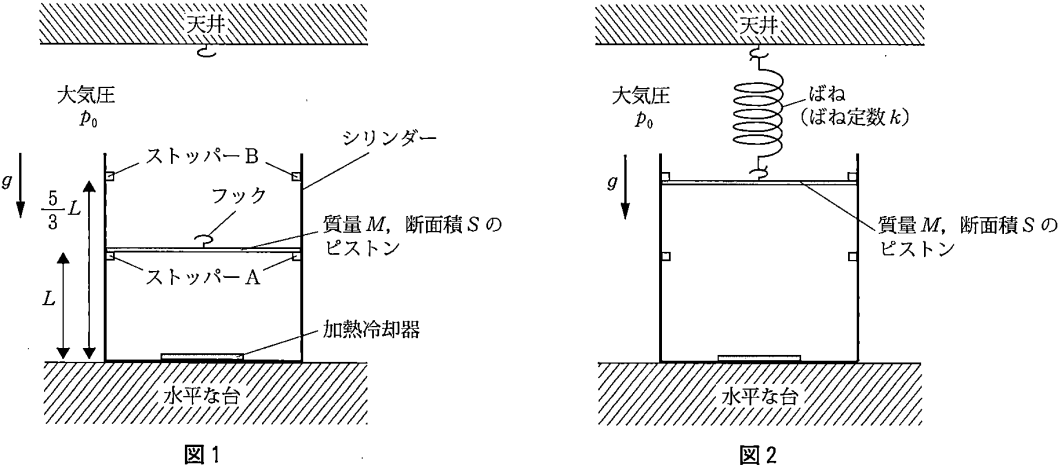
\includegraphics[width=\columnwidth]{../graphs/ko_riko_23_3.png}
\end{figure}


% メモ
\begin{comment}

\end{comment}


%%%%%%%%%%%%%%%%%%
